\documentclass{article}
\usepackage{graphicx} % Required for inserting images

\title{HPC-Master.Lab5}
\author{Thanh Bình Phan}
\date{October 2026}

\setlength{\parindent}{0pt}
\setlength{\parskip}{3pt}

\begin{document}


\maketitle

\section{Introduction}
This labwork is about implementing the Gaussian Blur filter running on GPU environment and examine the speedup when using \textit{shared memory} for that filter's kernel.
The image chosen is same as previous labworks.
\paragraph{Kernel} The whole labwork will be using the same $7*7$ kernel, which the values already computed in the slides, I just normalize it so that when applying the kernel, no need for additional division in the end. Note that I chose the data type to be \textit{float32} to be compatible with the shared memory kernel later on
\begin{verbatim}
hostKernel = np.array([
    [  0,   0,   1,   2,   1,   0,   0],
    [  0,   3,  13,  22,  13,   3,   0],
    [  1,  13,  59,  97,  59,  13,   1],
    [  2,  22,  97, 159,  97,  22,   2],
    [  1,  13,  59,  97,  59,  13,   1],
    [  0,   3,  13,  22,  13,   3,   0],
    [  0,   0,   1,   2,   1,   0,   0]
], np.float32)
hostKernel = hostKernel / hostKernel.sum()
KSIZE = hostKernel.shape[0]
\end{verbatim}

\paragraph{Convolution Operation} The idea is to get the neighborhood of the current pixel's position to the same size as the kernel, then multiple that subarray with the kernel element-wise, then take the sum. Formula below, where $dst$ and $src$ are the destination and source image, $y,x$ are the position of the pixel in the image, $k = floor(kernel\_size / 2)$.
\[
dst(y,x) = \sum_{dy=-k}^{k} \sum_{dx=-k}^k src(y+dy,x+dx) * kernel(dy+k, dx+k)
\]

For the edge pixels where some neighborhood pixels cannot be gotten, the strategy used in this labword is to assume that they are 0s, i.e. 0 padding technique.

\section{Gaussian Blur Implementation}
Below is my implementation code, without shared memory.
\begin{verbatim}
@cuda.jit
def gaussBlur(src, dst, kernel):
    # src and dst are in C, H, W shape
    c    = cuda.threadIdx.x + cuda.blockIdx.x * cuda.blockDim.x
    tidy = cuda.threadIdx.y + cuda.blockIdx.y * cuda.blockDim.y
    tidx = cuda.threadIdx.z + cuda.blockIdx.z * cuda.blockDim.z

    k = KSIZE // 2

    v = 0.0
    for dy in range(-k, k+1):
        for dx in range(-k, k+1):
            exists = ((tidx + dx) >= 0) & ((tidy + dy) >= 0)
            idx = min(max(tidx + dx, 0), W-1)
            idy = min(max(tidy + dy, 0), H-1)
            v += (exists * src[c, idy, idx]) * kernel[dy + k, dx + k]
    
    dst[c, tidy, tidx] = np.uint8(v)
\end{verbatim}

\paragraph{Changes compare to 2d gray scale} So there are some changes compared to the 2d grayscale function.
Firstly, the function signature takes an additional argument for the Gaussian kernel.
Secondly, $src$ and $dst$ (source and destination image respectively) now got reshaped into $C, W, H$, meaning instead of an 2D arrays of 3 values pixels, we have an array of 3 elements and each elements represents a RGB channel of the image.
The reason behind this is because I want to optimize the memory access for the convolution operation as the convolution has to be applied to each RGB channel independently and each operation will require the access to the neighborhood pixels values so making them closer in memory reduce the random access.

\paragraph{Some implementation details}
\begin{enumerate}
\item \textit{threadIdx.[xyz]} is not like what is said in the slide, or not according to my understanding of the slide. \textit{.x} is the outermost iteration, then \textit{.y} and \textit{.z}, from the slide I thought it was the other way around. So as seen in the code, \textit{tidx} should be gotten from \textit{.z}
\item I think of a trick to handle the edge pixels case without using \textit{if/else} statements. So there is an \textit{exists} variable which specify whether the neighborhood inbound or not. This variable will be added to the multiplication between the source and the kernel so that outbound pixels result is $0$. But if a pixel position is out of bound, we cannot get the value for the multiplication, so that's why $idx, idy$ is created to give a valid position.
\end{enumerate}

\paragraph{Shared memory} The shared memory version is similar, with these additional codes at the beginning. To illustrate simply, we create a \textit{'shared'} kernel in the shared memory between threads in a block, which should be a direct copy from the kernel in the global memory. Notice the $cuda.syncthreads()$ line to ensure all threads wait for the completion of the shared kernel creation.
\begin{verbatim}
s_kernel = cuda.shared.array((KSIZE, KSIZE), cuda.float32)
for y in range(KSIZE):
    for x in range(KSIZE):
        s_kernel[y, x] = kernel[y, x]
cuda.syncthreads()
\end{verbatim}
The kernel referenced by the code below all change to this shared kernel variable.

\section{Block Sizes Experiment}
The list of block sizes used is the same as the previous labwork: permutations of powers of two.
Each block size is run for 30 times then takes the average time.
The image only got scaled up by 2 each size this time due to the running time has significantly increase with the convolution operation.
Below is the comparison graph.

\begin{figure}[h]
    \centering
    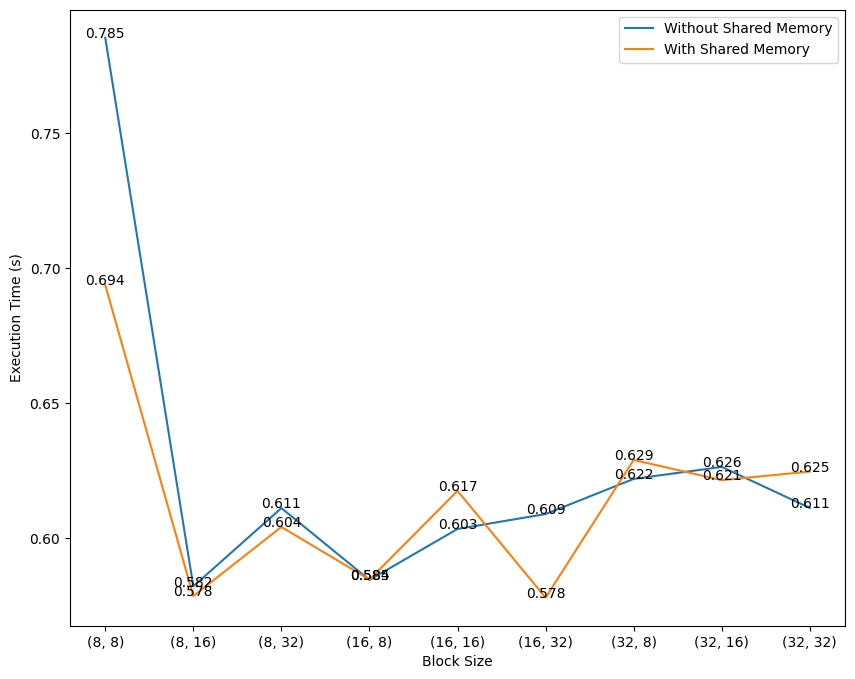
\includegraphics[width=0.7\linewidth]{blocksize-compare.png}
    \caption{Block Sizes Comparison, With(out) Shared Memory}
    \label{fig:blocksize-compare}
\end{figure}

So sadly, no considerable improvements as the theory said it should be, most block size values show really close execution time except for $(8,8)$ and $(16, 32)$.
My intial expectation is that the greater the block size, the more improvement that the shared memory version will show as more threads will use the fast shared memory, the time takes to copy from global memory to shared memory is constant with whatevery block size value used.

\end{document}
